\documentclass[UTF8]{ctexart}
\ctexset { section = { format={\Large \bfseries } } }
\pagestyle{plain}
\usepackage{float}
\usepackage{amsmath}
\usepackage{amssymb}
\usepackage{listings}
\usepackage{graphicx}%插入图片宏包
\usepackage{xcolor}
\usepackage{geometry}
\geometry{a4paper,scale=0.8}
\usepackage{caption}
\usepackage{subcaption}
\captionsetup[figure]{name={Figure}}
\captionsetup[table]{name={Table}}


\lstset{
language=Python, % 设置语言
basicstyle=\ttfamily, % 设置字体族
breaklines=true, % 自动换行
keywordstyle=\bfseries\color{blue}, % 设置关键字为粗体,
morekeywords={}, % 设置更多的关键字,用逗号分隔
emph={self}, % 指定强调词,如果有多个,用逗号隔开
emphstyle=\bfseries\color{Rhodamine}, % 强调词样式设置
commentstyle=\color{black!50!white}, % 设置注释样式,斜体,浅灰色
stringstyle=\bfseries\color{red!90!black}, % 设置字符串样式
columns=flexible,
numbers=left, % 显示行号在左边
numbersep=2em, % 设置行号的具体位置
numberstyle=\footnotesize, % 缩小行号
frame=single, % 边框
framesep=1em % 设置代码与边框的距离
}

\title{\textbf{Image Processing Homework 2}}
\author{吴嘉骜 21307130203}
\date{\today}

\begin{document}

\maketitle

\noindent
\section{}
\setlength{\parindent}{0pt}
Restate the Basic Global Thresholding (BGT) algorithm so that it uses the histogram of an image instead of the image itself. (Please refer to the statement of OTSU algorithm)\\
\textbf{Solution}:\\
The BGT based on the histogram can be stated as below.\\
1. Select an initial threshold $T_0$, such as the mean intensity.\\
2. Partition the histogram into two classes: $R_1$ with intensity values $[0, T_{i-1}-1]$ and $R_2$ with intensity values $[T_{i-1}, L - 1]$, where $L$ is the number of intensity levels in the image.\\
3. Calculate the mean intensity values $\mu_{[0,T_{i-1}-1]}$ and $\mu_{[T_{i-1},L-1]}$ of the partitions $R_1$ and $R_2$ by using the following equations:\\
\begin{equation*}
    \mu_{[0,T_{i-1}-1]} = \frac{\sum\limits_{j=0}^{T_{i-1}-1} j p(j)}{\sum\limits_{j=0}^{T_{i-1}-1} p(j)}
\end{equation*}

\begin{equation*}
    \mu_{[T_{i-1},L-1]} = \frac{\sum\limits_{j=T_{i-1}}^{L-1} j p(j)}{\sum\limits_{j=T_{i-1}}^{L-1} p(j)}
\end{equation*}
where $p(j) = \frac{n_j}{N}$ is the $j$th element of the normalized histogram.\\
4. Calculate the new threshold value $T_i = (\mu_{[0,T_{i-1}-1]}+\mu_{[T_{i-1},L-1]})/2$.\\
5. Repeat Steps 2 through 4 for $i = 1,2,\ldots$, until $|T_i - T_{i-1}| \leq \epsilon$, a predefined tolerance value.\\

\section{}
Design an algorithm of locally adaptive thresholding based on local OTSU or maximum of local entropy; implement the algorithm and test it on exemplar image(s).\\
\textbf{Solution}:\\
The locally adaptive thresholding based on local OTSU can be stated as below.\\
1. Determine the size of the local window $W \times W$ as the neighborhood of each pixel.\\
2. For each pixel $(x,y)$ in the image, calculate the optimal threshold $T(x,y)$ using OTSU algorithm based on the local histogram centered at $(x,y)$.\\
3. Threshold the center of the window by $T(x,y)$.\\
4. Repeat Steps 2 and 3 for each pixel in the image, until all pixels have been processed.\\
Details of Step 2 are listed below.\\
(a). Calculate the normalized histogram $h(x,y)$ of the local $W \times W$ window centered at $(x,y)$.\\
(b). Calculate the average intensity of the entire image by $m_G = \sum\limits_{i=0}^{L-1} i p_i$.\\
(c). For each threshold $T(k)= k \in (0,L-1)$, where $L$ is the number of intensity levels in the image, 
calculate the cumulative sum $P_1(k)$ of class 1 by $P_1(k) = \sum\limits_{i=0}^{k} p_i$.\\
(d). Calculate the cumulative mean up to level k by $m(k) = \sum\limits_{i=0}^{k} i p_i$.\\
(e). Calculate the between-class variance $\sigma_B^2(k) = \frac{(m_GP_1(k)-m(k))^2}{P_1(k)(1-P_1(k))}$.\\
(f). Pick the optimal threshold $T(x,y)$ which is the value of $k$ that maximizes $\sigma_B^2(k)$.\\

The code is shown below. See details in \texttt{thres\_otsu.py}.
\begin{lstlisting}
    from PIL import Image

    def compute_otsu_threshold(hist):
        """
        Compute Otsu's threshold for a given histogram.
        
        Input:
            - hist: a histogram (a dictionary), where the key is the pixel value and the value is the frequency of that pixel value.
            
        Output:
            - threshold: the optimal threshold value.
        """
        # If only one value in histogram
        if len(hist) == 1:
            return 0 if next(iter(hist)) < 128 else 255
        
        #  extract the sorted keys from the histogram
        keys = sorted(hist.keys())
        
        #  compute the total number of pixels in the neighborhood
        total = sum(hist.values())
        
        # the mean of the image
        mG = sum([i * hist[i] for i in hist])/ total
        
        # initialize the variables
        var_between = 0
        threshold = 0
        max_var = -float('inf')
        best_ks = []  # list to store all k values with max variance
        p1_cumulative = 0
        m_cumulative = 0
    
        for index in range(0, len(keys)-1):
            k = keys[index]
            post_k = keys[index + 1]
            
            # Update the cumulative sums for the next iteration
            p1_cumulative += hist[k] / total
            m_cumulative += k * hist[k] / total
            
            p1 = p1_cumulative  # the weight background
            m = m_cumulative  #  the cumulative mean background
            if p1 == 0 or p1 == 1:
                continue
            
            # Check if the current variance is greater than max_var
            var_between = (mG*p1-m)**2/(p1*(1-p1))  # the variance between classes
            if var_between > max_var:
                max_var = var_between
                best_ks = [i for i in range(k, post_k)]
            elif var_between == max_var:
                best_ks = best_ks + [i for i in range(k, post_k)]
            
        # Compute the average threshold from all best k values
        if len(best_ks) > 0:
            threshold = sum(best_ks) / len(best_ks)
        return threshold
    
    
    def adaptive_otsu(img_path, W):
        '''
        Adaptive Otsu's thresholding algorithm.
        
        Input:
            - img_path: the path to the image.
            - W: the window size, an odd number. Default is 3.
            
        Output:
            - output: the binarized image.
        '''
        from localhistW_compute import local_histogram
    
        local_histograms = local_histogram(img_path, W)
        
        img = Image.open(img_path)
        if img.mode != 'L':
            img = img.convert('L')
    
        width, height = img.size
        pixels = img.load()
    
        output = Image.new('L', (width, height))
        output_pixels = output.load()
    
        for i in range(height):
            for j in range(width):
                threshold = compute_otsu_threshold(local_histograms[i][j])
                if threshold == 0:
                    output_pixels[j, i] = 0
                elif threshold == 255:
                    output_pixels[j, i] = 255
                else:
                    output_pixels[j, i] = 255 if pixels[j, i] > threshold else 0
    
        return output
\end{lstlisting}
\textbf{Code interpretation}:\\
The code above defines two functions.\\
The first function \textbf{compute\_otsu\_threshold} is used to compute the optimal threshold value for a given histogram. Note that if
the histogram only has one value, the threshold is set to 0 if the value is less than 128, otherwise 255. If the histogram has more than one value, the threshold is computed by the OTSU algorithm.\\
The second function \textbf{adaptive\_otsu} is used to implement the locally adaptive thresholding based on local OTSU. 
When binarizing, if the threshold is 0, the pixel intensity is set to 0; if 255, the intensity is set to 255. Otherwise, the pixel is set to 255 if the pixel value is greater than the threshold, otherwise 0.\\
\textbf{Test result}:\\
We test the algorithm on a text image corrupted by spot shading, which has been shown in class. The original image and binarized ones are shown below.\\
\begin{figure}[htbp]
    \centering
    % 第一行三张图片
    \begin{subfigure}{0.3\textwidth}
        \centering
        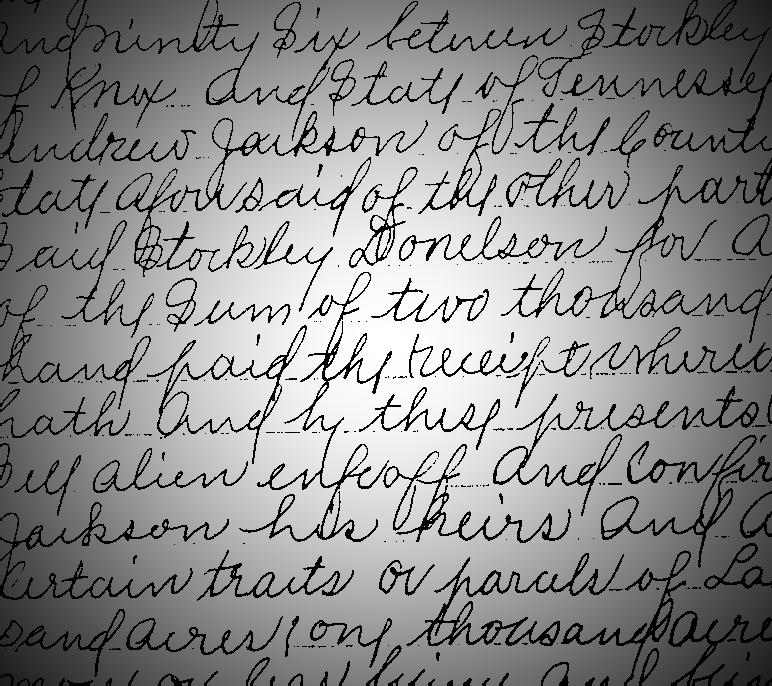
\includegraphics[width=\linewidth]{spot_shaded_text_image.jpg}
        \caption{Input original image}
    \end{subfigure}%
    \hfill
    \begin{subfigure}{0.3\textwidth}
        \centering
        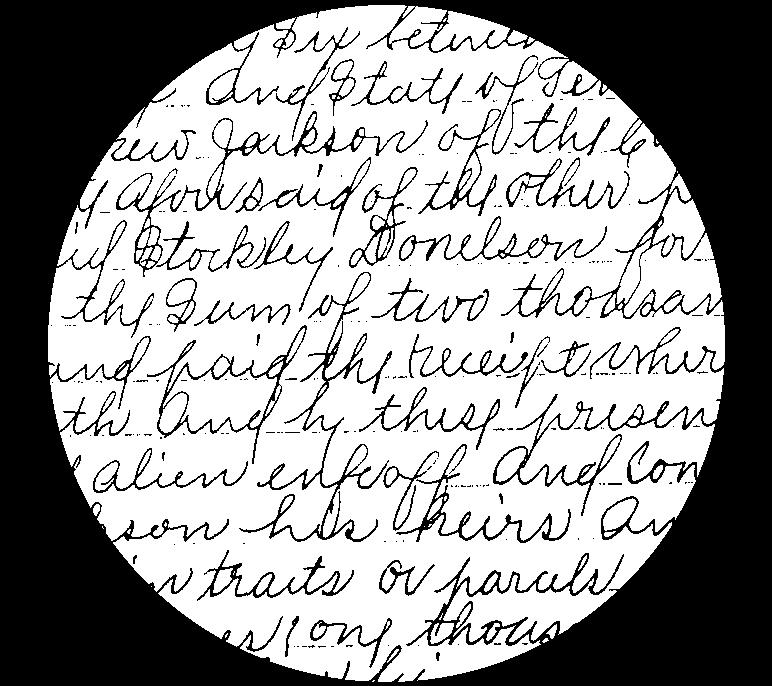
\includegraphics[width=\linewidth]{global_otsu.jpg}
        \caption{Global OTSU}
    \end{subfigure}%
    \hfill
    \begin{subfigure}{0.3\textwidth}
        \centering
        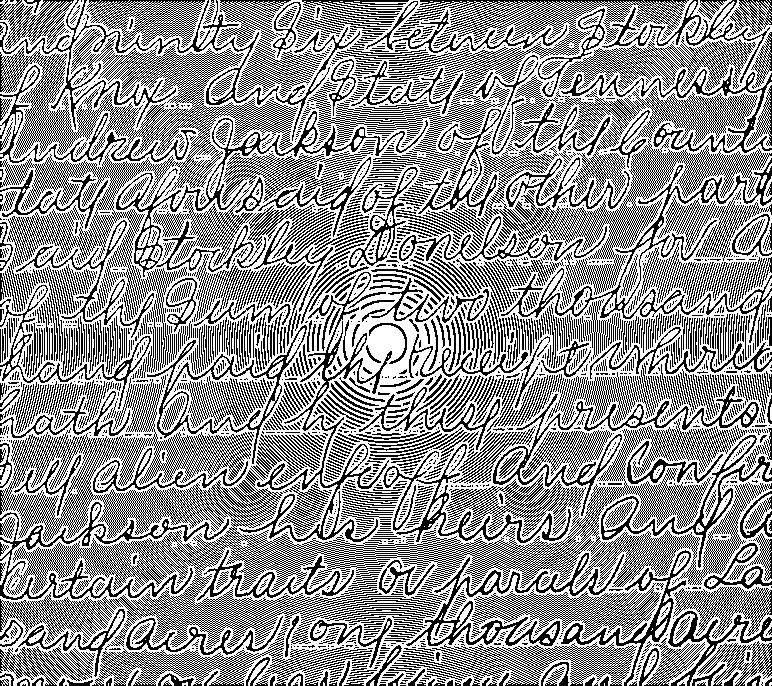
\includegraphics[width=\linewidth]{local_otsu5.jpg}
        \caption{Local OTSU window size 5}
    \end{subfigure}

    \vspace{0.5cm} % 调整两行之间的距离

    % 第二行三张图片
    \begin{subfigure}{0.3\textwidth}
        \centering
        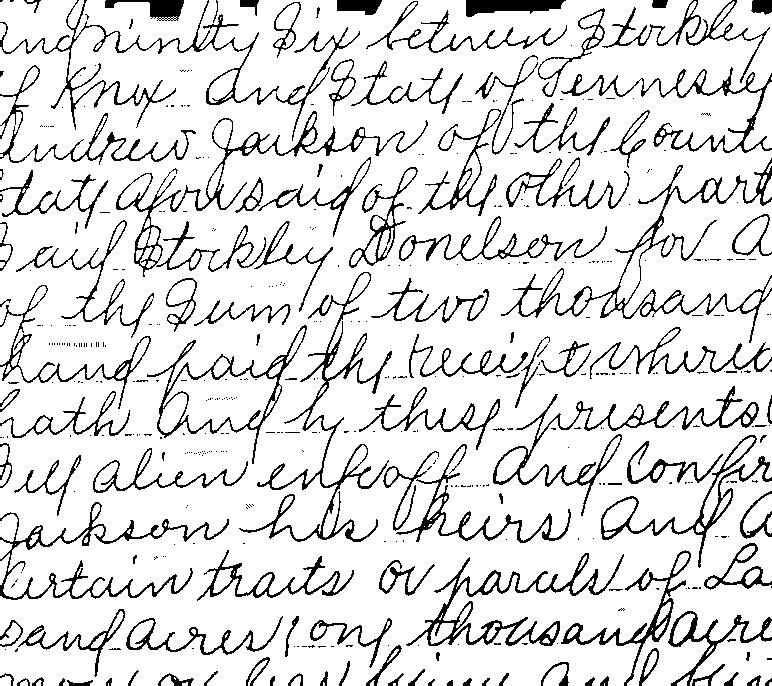
\includegraphics[width=\linewidth]{local_otsu35.jpg}
        \caption{Local OTSU window size 35}
    \end{subfigure}%
    \hfill
    \begin{subfigure}{0.3\textwidth}
        \centering
        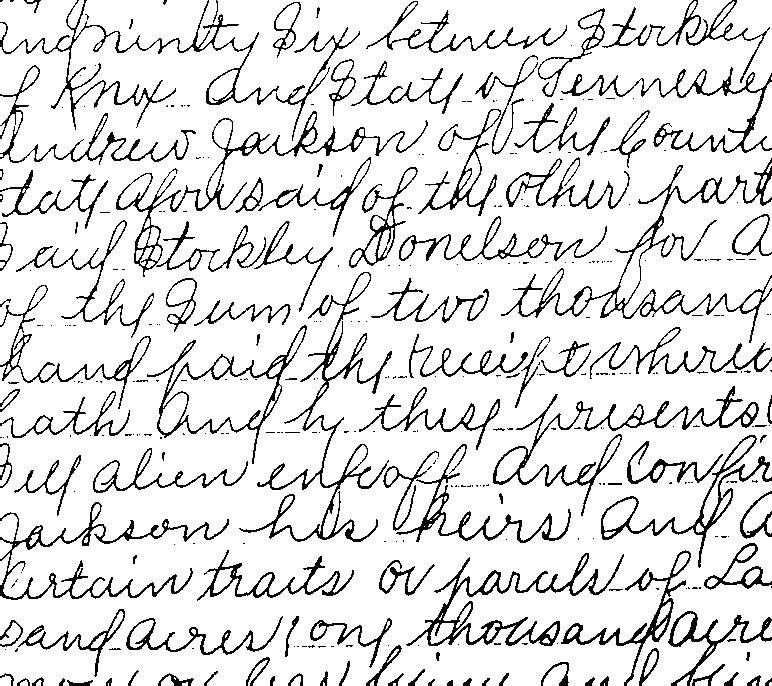
\includegraphics[width=\linewidth]{local_otsu65.jpg}
        \caption{Local OTSU window size 65}
    \end{subfigure}%
    \hfill
    \begin{subfigure}{0.3\textwidth}
        \centering
        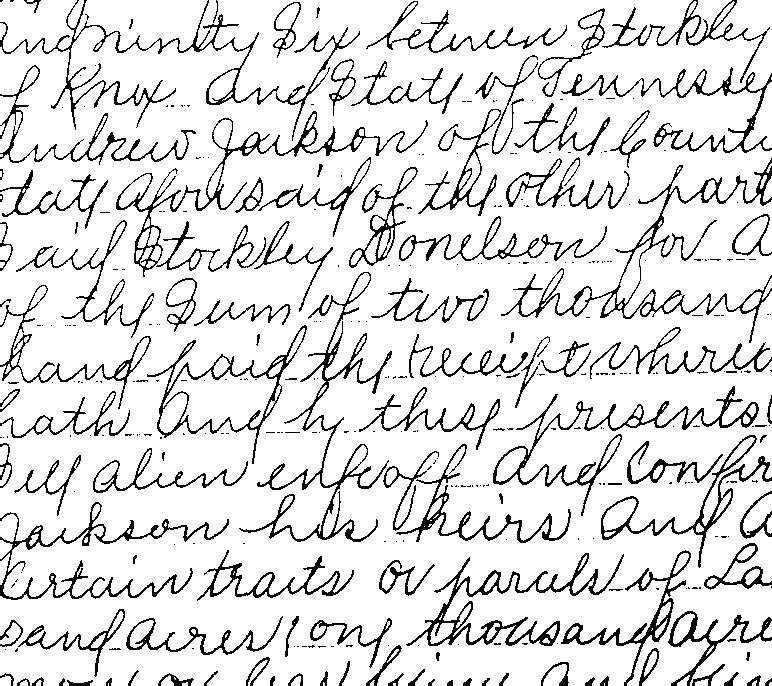
\includegraphics[width=\linewidth]{thresh0.jpg}
        \caption{Threshold = 0}
    \end{subfigure}

    \caption{Image after OTSU thresholding}
\end{figure}

\textbf{Analysis}:\\
The original image is embedded in a nonuniform illumination field, which is caused by spot shading.\\
The global OTSU algorithm cannot overcome this problem well, and the binarized image is not satisfactory.\\
The effect of local OTSU algorithm proves to be better than the global one, but depends largely on the window size of the local histogram.
As shown in the figure above, when the window size is small (e.g. 5), there is so much annular noise in the background that it is difficult to 
distinguish between foreground and background.\\
When the window size gets larger, the binarized image is better, but still has black blocks above the text (e.g. window size 35).\\
When the window size is large enough (e.g. 65), the binarized image is satisfactory and the algorithm turns out to be effective.\\
The reason is probably that with a rather small window size, the noises in the background dominate the local histogram, which leads to a bad threshold value. 
When the window size gets larger, the foreground can be distinguished clearly from the background, and the threshold value is more accurate.\\
Finally, if we simply set the threshold to 0, which means only the handwritten text is preserved, the result is also satisfactory. This is not a surprising result
because the background is strictly white with positive intensities.
And the last method is much faster than the local OTSU algorithm.\\

\section{}
Implement linear interpolation algorithm (do not call the interpolation function in some library), and apply: read out an image, use linear interpolation to enlarge the spatial resolution of the picture $N$ times, and then save the picture.\\
\textbf{Solution}: 
The code is shown below. See details in \texttt{linear\_interpolation.py}.
\begin{lstlisting}
    from PIL import Image

def linear_interpolation(val1, val2, alpha):
    '''
    Linear interpolation between val1 and val2
    
    Input:
        - val1: value 1
        - val2: value 2
        - alpha: interpolation factor
        
    Output:
        - interpolated value
    '''
    return val1 * (1 - alpha) + val2 * alpha

def resize_image(img_path, scale=1):
    '''
    Resize the image with the given scale
    
    Input:
        - img_path: path to the image
        - scale: scale factor
        
    Output:
        - resized image
    '''
    #  Open the image and convert to grayscale
    img = Image.open(img_path).convert('L')
    width, height = img.size
    
    #  Calculate the new image size
    new_width = int(width * scale)
    new_height = int(height * scale)

    new_img = Image.new('L', (new_width, new_height))
    original_pixels = img.load()
    new_pixels = new_img.load()

    for x in range(new_width):
        for y in range(new_height):
            #  Map the pixel from new image to original image
            #  gx, gy: new pixels' coordinates in original image
            gx = x / scale
            gy = y / scale

            #  Get the coordinates of the 4 pixels around the new pixel
            gx0 = int(gx)
            gy0 = int(gy)
            gx1 = min(gx0 + 1, width - 1)
            gy1 = min(gy0 + 1, height - 1)

            #  Calculate the alpha values for interpolation
            alpha_x = gx - gx0
            alpha_y = gy - gy0

            # Linear interpolation in x direction
            val_y0 = linear_interpolation(original_pixels[gx0, gy0], original_pixels[gx1, gy0], alpha_x)
            val_y1 = linear_interpolation(original_pixels[gx0, gy1], original_pixels[gx1, gy1], alpha_x)


            # Linear interpolation in y direction
            value = int(linear_interpolation(val_y0, val_y1, alpha_y))
            new_pixels[x, y] = max(0, min(255, value))  # Clamp the value to [0, 255]

    return new_img
\end{lstlisting}
\textbf{Code interpretation}:\\
The code above defines two functions.\\
The first function \textbf{linear\_interpolation} is used to compute the interpolated value between two values.\\
The second function \textbf{resize\_image} is used to resize the image with the given scale. First we initialize a new image with the new size,
and map the pixels $(x,y)$ in the new image to the original image $(gx,gy)$ by scaling. Then we find the 4 pixels around $(gx,gy)$ in the original image.
The left-top pixel is $(gx_0,gy_0)$, and the right-bottom pixel is $(gx_1,gy_1)$. Last, we calculate the interpolated value by linear interpolation in first x and then y directions.
After all pixels in the new image have been processed, we return the new image.\\
\textbf{Test result}:\\
We test the algorithm in the following way. First we shrink the original image with 1250 dpi to 125 dpi by scaling it to $\frac{1}{10}$ of the original size.
Then we zoom the shrinked image back to 1250 dpi by scaling it 10 times.
The original, shrinked and enlarged images are shown below.\\
\begin{figure}[htbp]
    \centering
    % 第一行三张图片
    \begin{subfigure}{0.3\textwidth}
        \centering
        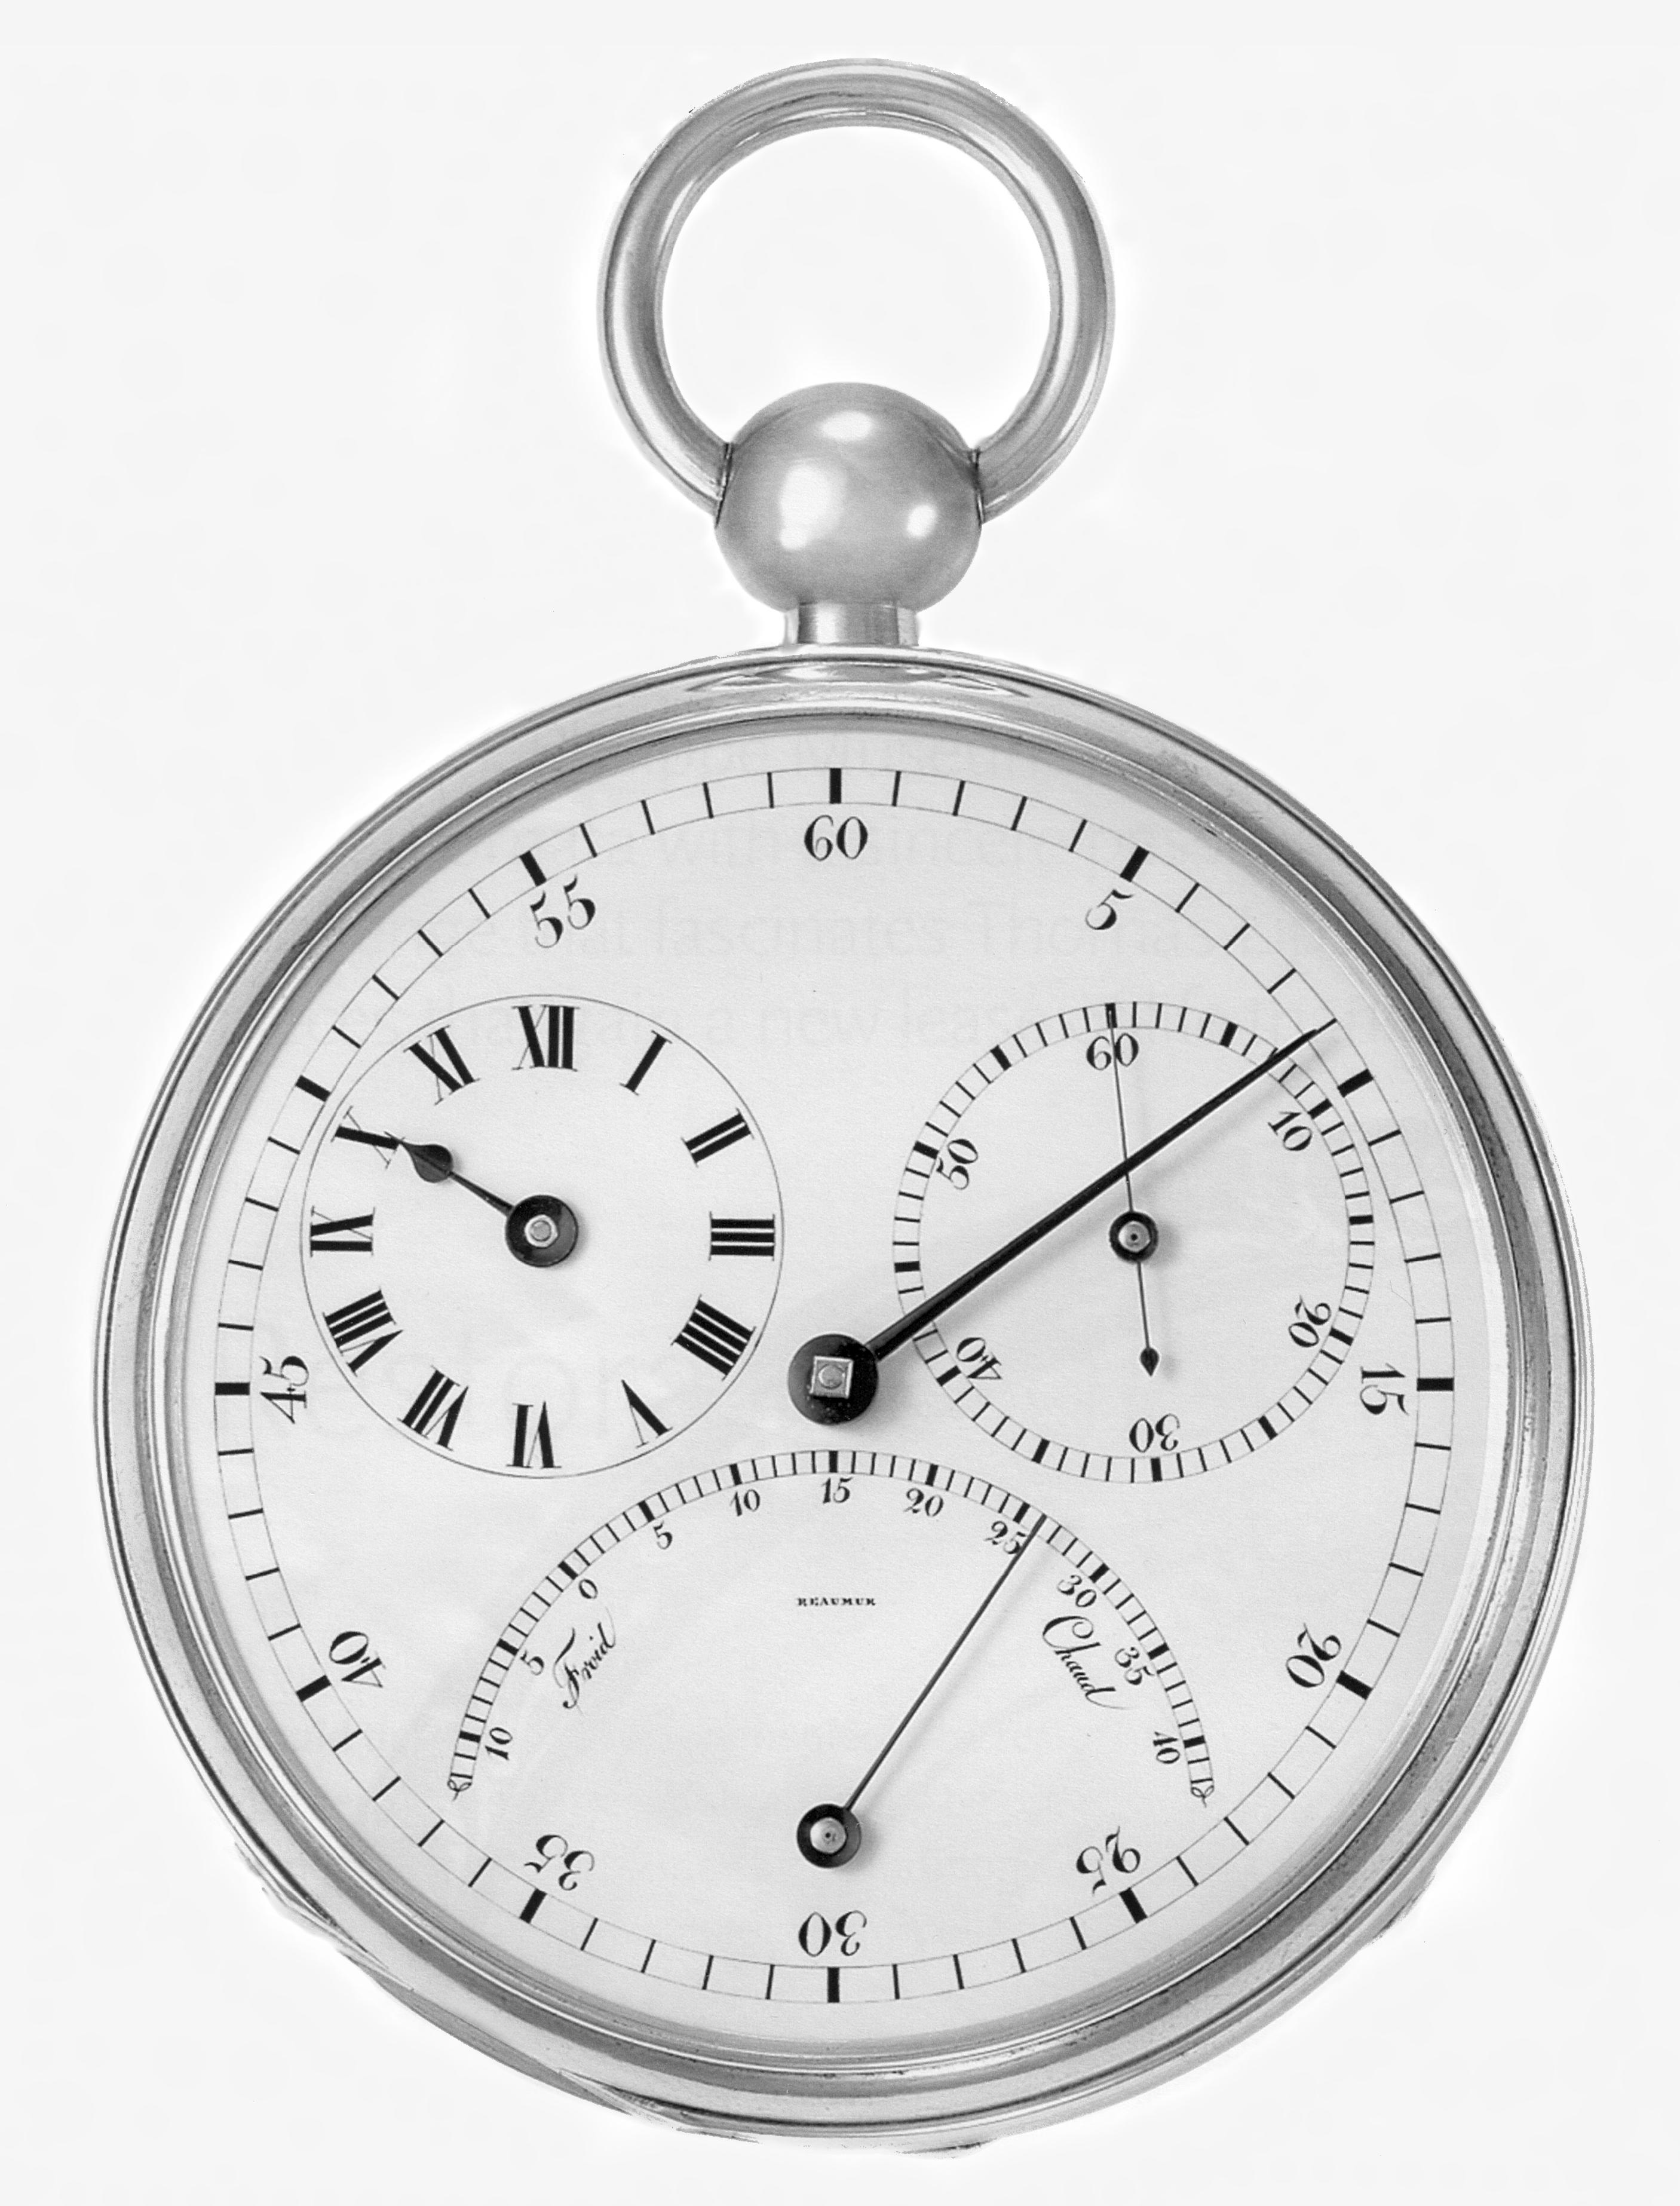
\includegraphics[width=\linewidth]{chronometer 1250 dpi.jpg}
        \caption{Original image with 1250 dpi}
    \end{subfigure}%
    \hfill
    \begin{subfigure}{0.3\textwidth}
        \centering
        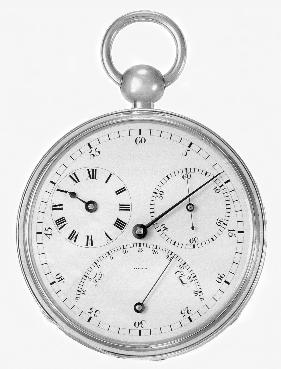
\includegraphics[width=\linewidth]{shrinked_image.jpg}
        \caption{Shrinked image with 125 dpi}
    \end{subfigure}%
    \hfill
    \begin{subfigure}{0.3\textwidth}
        \centering
        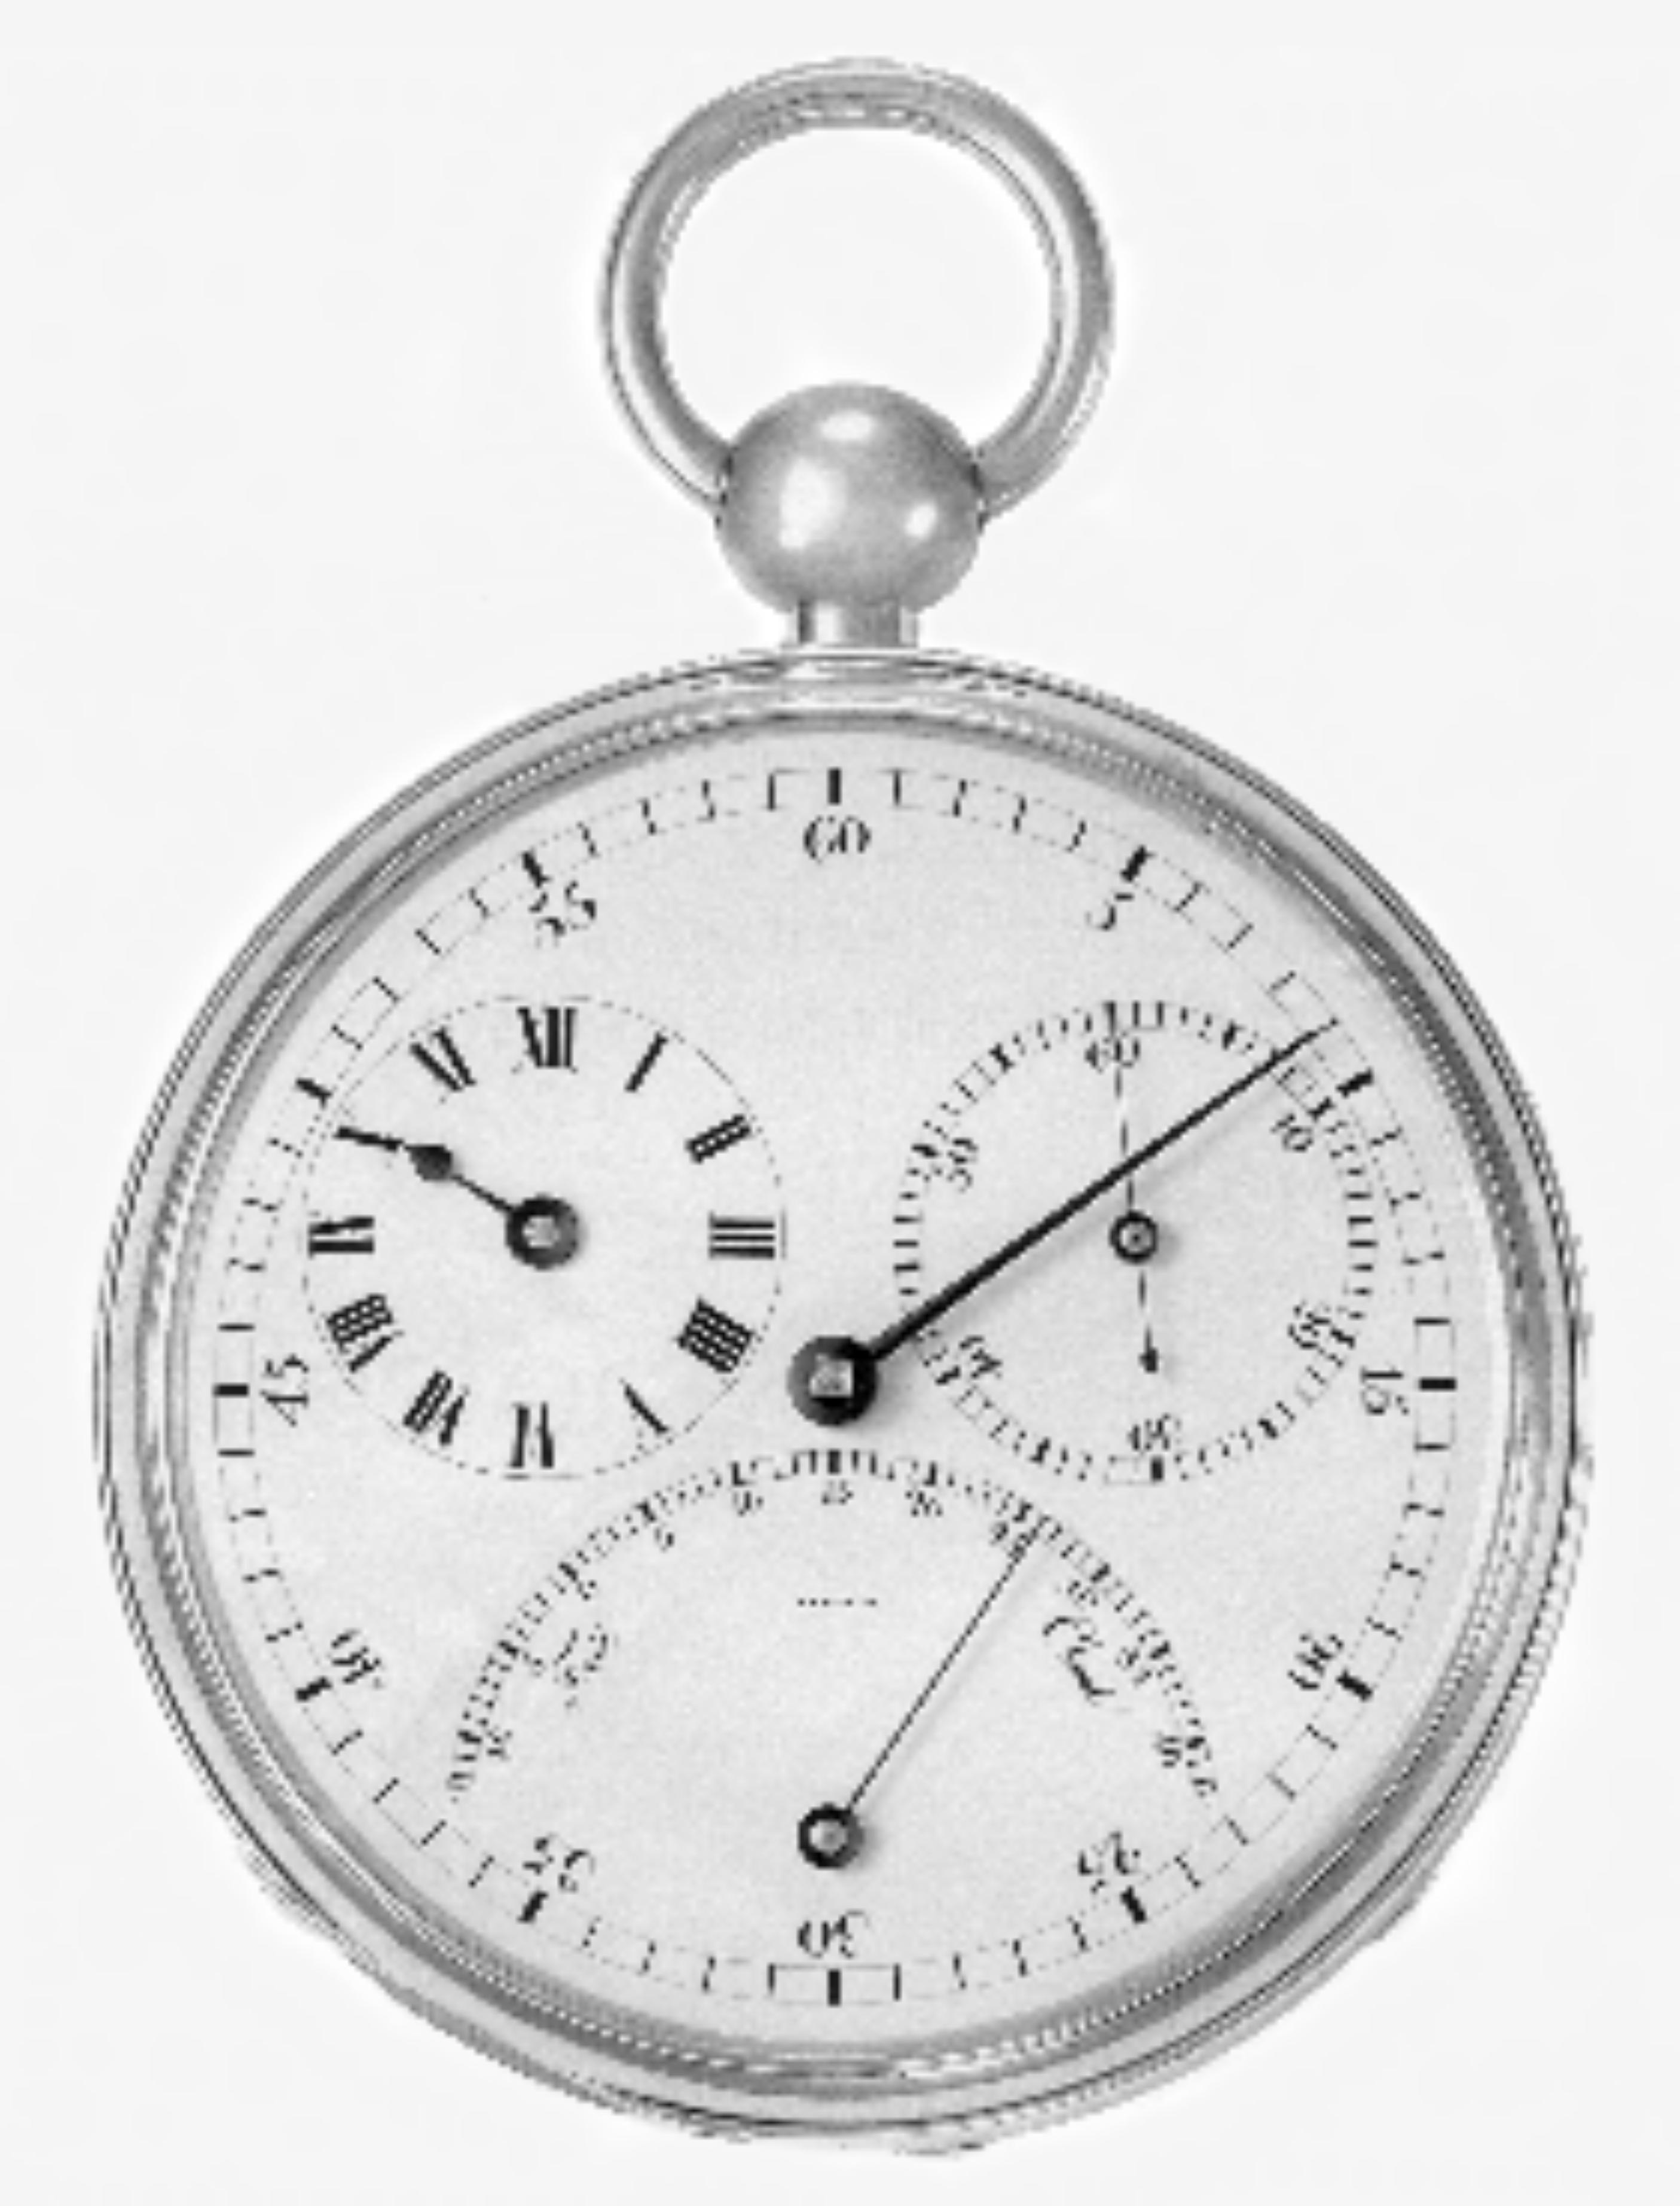
\includegraphics[width=\linewidth]{shrinked_zoomed_image.jpg}
        \caption{Enlarged image with 1250 dpi}
    \end{subfigure}

    \caption{Image after linear interpolation}
\end{figure}

\textbf{Analysis}:\\
After shrinking the image, the image is blurred snd show degraded quality. 
This is because the pixels in the original image are averaged to get the new pixel value, but with a reduced spatial resolution.\\
By resizing the shrinked image, the image seems to be clearer and sharper, but still not as good as the original one.
This is probably because linear interpolation is a basic method, losing more details than other advanced methods, such 
as bicubic interpolation.\\

\end{document}